\textbf{APRAKSTOŠĀ STATISTIKA}

\equationEntry{Vidējais aritmētiskais:}
{\begin{align*}
     AVERAGE(Arr) = \overline{x} &= \frac{\sum{i=1}{n}x_i}{0} \\
\end{align*}}

\equationEntry{Mediānas pozīcija:}
{\begin{align*}
    MEDIAN(Arr) = \frac{n+1}{2}
\end{align*}}

\equationEntry{Ģeometriskais vidējais:}
{\begin{align*}
    \overline{x} &= \sqrt[n]{x_1*x_2*\dots*x_n} \\
    \overline{x} &= GEOMEAN(number1, [number2], ...)
\end{align*}}

\equationEntry{Amplitūda (rangs):}
{\begin{align*}
    range(X)=X_{max}-X_{min}
\end{align*}}

\equationEntry{Dispersija (variance) izlasei:}
{\begin{align*}
    s^2 &= VAR.S(X) \\
    s^2 &= \frac{\sum_{i=0}^{n} (x_i-\overline{x})^2}{n-1}
\end{align*}}

\equationEntry{Dispersija (variance) ģenerālkopai:}
{\begin{align*}
    \sigma^2 &= VAR.P(X) \\
    \sigma^2 &= \frac{\sum_{i=0}^{n} (x_i-\overline{x})^2}{N}
\end{align*}}

\equationEntry{Standartnovirze (standartkļūda) izlasei:}
{\begin{align*}
    s &= STDEV.S(X) \\
    s &= \sqrt{s^2} \\
\end{align*}}

\equationEntry{Standartnovirze (standartkļūda) ģenerālkopai:}
{\begin{align*}
    s &= STDEV.P(X) \\
    \sigma &= \sqrt{\sigma^2}
\end{align*}}



\equationEntry{Standartizētā vērtība (Z-score):} 
{\begin{align*}
    Z &= \frac{x-\overline{x}}{s} \\
    Z &= \frac{x-\overline{x}}{\sigma}
\end{align*}}

\equationEntry{Asimetrijas koeficients:}
{

    \vspace*{.1in}
    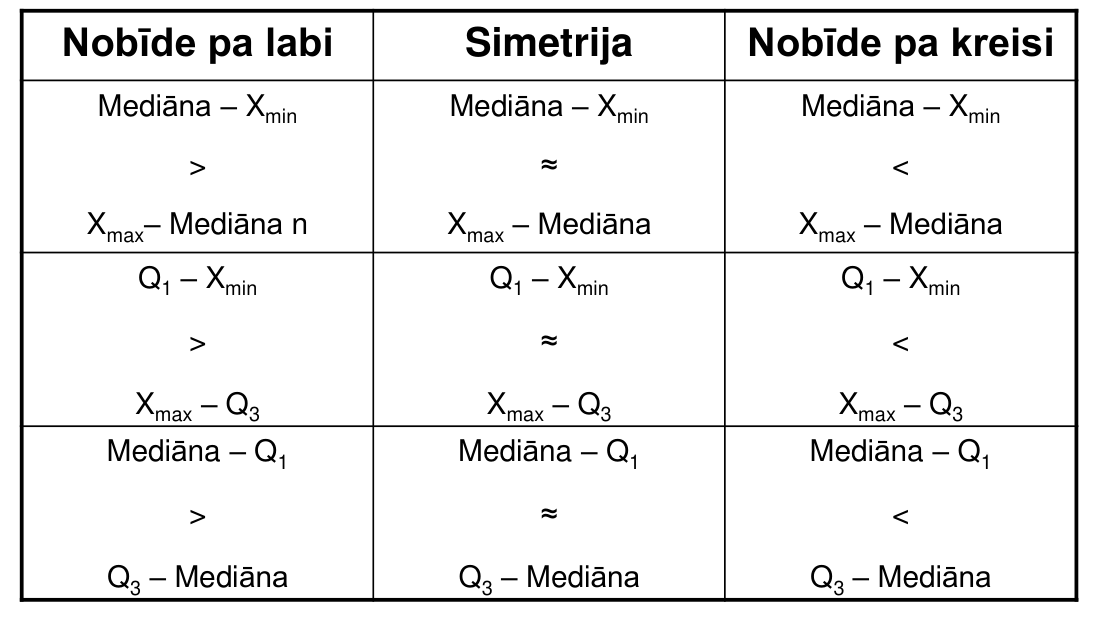
\includegraphics[width=1\textwidth]{SymmetryTable}
}

\equationEntry{Kvartiles:}

{

    If we have an ordered dataset $ x_{1},x_{2},...,x_{n}$, we can interpolate
    between data points to find the p pth empirical quantile if $x_{i}$ is in
    the ${\displaystyle i/(n+1)}$ quantile. If we denote the integer part of a
    number $a$ by $\lfloor a\rfloor$ , then the empirical quantile function is
    given by,

    \begin{align*}
        q(p/4) &= x_k + \alpha ( x_{k + 1} - x_k ) = QUARTILE.EXC(Arr, p) \\
        k &=\lfloor p(n+1)/4\rfloor \\
        \alpha &=p(n+1)/4-\lfloor p(n+1)/4\rfloor
    \end{align*}

    To find the first, second, and third quartiles of the dataset we would
    evaluate $q(0.25), q ( 0.5 ) q(0.5), and q ( 0.75 ) q(0.75)$ respectively. 

}

\equationEntry{Starpkvartiļu rangs (IQR):}
{
    \begin{align*}
        IQR &= Q_3-Q_1
    \end{align*}
}


\equationEntry{Kastes diagramma (Box plot)}
{
    \vspace*{.1in}
    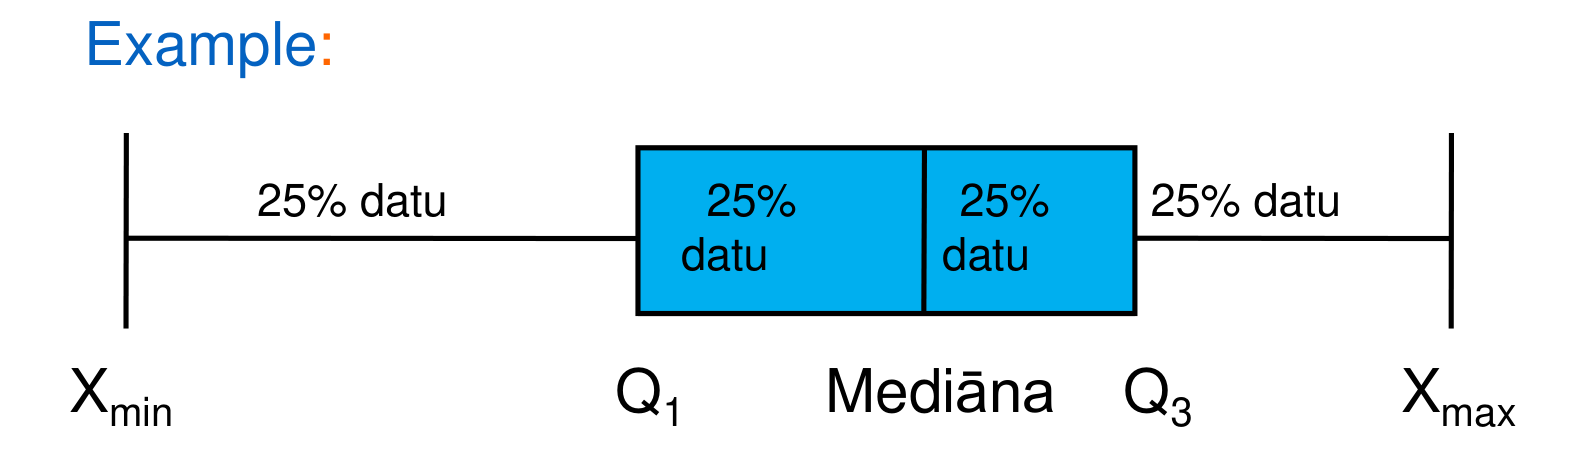
\includegraphics[width=1\textwidth]{BoxPlot}
}

\equationEntry{Kovariācija}
{
    \begin{align*}
        cov_s(X,Y) &= \frac{\sum_{i=0}^{n} (X_i-\overline{X})(Y_i-\overline{Y_i})}{n-1}' \\
        cov_p(X,Y) &= \frac{\sum_{i=0}^{n} (X_i-\overline{X})(Y_i-\overline{Y_i})}{n}' \\
        cov_s(X,Y) &= COVARIANCE.S(array1, array2) \\
        cov_p(X,Y) &= COVARIANCE.P(array1, array2)
    \end{align*}
}

\equationEntry{Kovariācijas koeficients (r; Pearson's)}
{
    \begin{align*}
        cov_s(X,Y) &= \frac{\sum_{i=0}^{n} (X_i-\overline{X})(Y_i-\overline{Y_i})}{n-1}' \\
        r = \displaystyle\frac{COV(x,y)}{\sigma_x \sigma_y} &= CORREL(array1, array2)
    \end{align*}
}
